\chapter{De MEGA65 upgraden}

\section{Hoe u een MEGA65 kunt upgraden}
\label{cha:cores}

Het MEGA65-platform bestaat uit drie belangrijke onderdelen:

\begin{enumerate}
  \item De {\bf MEGA65-core},\index{Core} een beschrijving van de chipset die op de FPGA draait  \item De {\bf ROM},\index{ROM} code die het besturingssysteem in Commodore-stijl (KERNAL) en BASIC definieert  \item {\bf Systeemsoftware} voor functies zoals het Freezer-menu\index{Freezer-menu}
\end{enumerate}

U kunt deze onderdelen upgraden zodra er nieuwe versies verschijnen. U kunt ook één of meer van deze onderdelen afzonderlijk vervangen. Bij de core en de ROM kunt u zelfs meerdere versies tegelijk geïnstalleerd hebben en daartussen schakelen. In plaats van de nieuwste MEGA65-ROM kunt u bijvoorbeeld overschakelen naar de originele prototype-ROM van de Commodore 65. Of u kunt overschakelen naar een andere core die ervoor zorgt dat uw MEGA65-hardware zich geheel als een andere computer gedraagt, zoals een Commodore 64 of een ZX Spectrum.

De ROM en de systeemsoftware zijn bestanden die op de SD-kaart staan; het upgraden ervan is even eenvoudig als het vervangen van de bestanden. Om de core te upgraden installeert u via een bepaald proces een core-bestand in het core-flashgeheugen van de MEGA65. Dit hoofdstuk beschrijft dit proces.

\subsection{Wat is een core?}
\index{Core!Wat is een core?}

De hardware-architectuur van de MEGA65 is gebaseerd op een veelzijdige chip die een ``Field Programmable Gate Array'' of FPGA wordt genoemd.\index{Field Programmable Gate Array (FPGA)} Dit is een speciaal soort computerchip die geprogrammeerd kan worden om zich als andere chips voor te doen. Het doet dit door een enorme reeks logische poorten zodanig te configureren dat de poorten schakelingen nabootsen. FPGA's zijn geen emulatie, maar een elektronische nabootsing van andere chips. FPGA-code wordt soms aangeduid als {\em firmware,} een term die u wellicht herkent van moderne computers en andere apparaten.

Uw MEGA65 is in de fabriek geprogrammeerd om een chipset na te bootsen die is gebaseerd op de originele Commodore 65 en door het MEGA65-team is ontworpen. U kunt de FPGA van de MEGA65 opnieuw programmeren om te upgraden naar nieuwe versies van de MEGA65-chipset of om de chipset te vervangen door die van een heel andere computer!

Elke mogelijke chipset wordt een {\em core} genoemd. De MEGA65 kan maximaal acht cores opslaan en u kunt tussen deze cores schakelen via een menu dat opent wanneer u de computer inschakelt. U kunt dit menu ook gebruiken om een nieuwe core vanaf een bestand op de SD-kaart te laden, een proces dat {\em flashen} heet.

Leden van de MEGA65-gemeenschap hebben diverse nuttige en leuke alternatieve cores voor de FPGA-hardware gemaakt. \href{https://github.com/MJoergen/C64MEGA65}{{\em C64 voor MEGA65}} van MJoergen en sy2002 bootst de originele Commodore 64-computer met een hoge mate van nauwkeurigheid na en is perfect voor het uitvoeren van Commodore 64-spellen, demo's en toepassingen. Andere cores bootsen de ZX Spectrum, de Game Boy en zelfs de hardware van de originele Galaga-arcademachine na. De FPGA van de MEGA65 is krachtig genoeg om vrijwel alle 8-bit-homecomputers na te bootsen en waarschijnlijk ook enkele 16-bit-computers en spelcomputers, zoals de Commodore Amiga. Het hardware-ontwerp van de MEGA65, de indeling van het moederbord, de FPGA-core en overige informatie zijn allemaal gratis beschikbaar onder diverse openbronlicenties, zodat iedereen vrij is andere cores voor de MEGA65-hardware te maken.

\section{De versies van de onderdelen bepalen}
\label{sec:versions}

Alle onderdelen van het MEGA65-platform hebben een versieaanduiding. De MEGA65 kan de versieaanduidingen van al zijn onderdelen weergeven met het MEGA65-informatiehulpprogramma.\index{MEGA65-informatiehulpprogramma}

Om het MEGA65-informatiehulpprogramma te openen:

\begin{enumerate}
  \item Schakel de MEGA65 in en laat hem opstarten tot BASIC.  \item Open de Freezer:\index{Freezer-menu} houd \widekey{RESTORE} één seconde ingedrukt en laat hem daarna los.  \item Druk op \specialkey{HELP}. Het MEGA65-informatiehulpprogramma opent.
\end{enumerate}

\begin{center}
  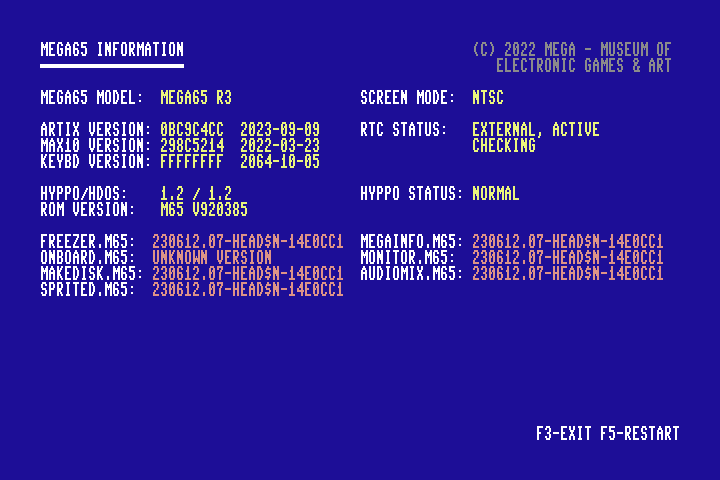
\includegraphics[width=0.7\linewidth]{images/megainfo.png}
\end{center}

Noteer deze versieaanduidingen:
\nopagebreak
\begin{center}
\setlength{\tabcolsep}{1mm}
\begin{tabularx}{\textwidth}{|X|p{7cm}|}
  \hline
  {\bf Label en voorbeeld} & {\bf Beschrijving} \\
  \hline
  MEGA65-model\newline {\tt MEGA65 R6} & De revisie van de hardware. U moet dit weten wanneer u nieuwe core-bestanden downloadt. \\
  \hline
  Artix-versie\index{Core!Versies}\newline {\tt 8AD00DD7 2024-01-22} & De MEGA65-core die op dit moment draait. Dit is een reeks van acht letters en cijfers en tevens een builddatum. \\
  \hline
  ROM-versie\index{ROM!Versie}\newline {\tt M65 V920393} & De ROM die op dit moment draait. Voor MEGA65-ROM's is dit een oplopend nummer, waarbij grotere nummers nieuwere versies aanduiden. \\
  \hline
  Systeembestanden (.M65)\newline {\tt 240122.21-R0.3.0-8B6C767} & Elk bestand van de systeemsoftware heeft een eigen versieaanduiding. Gewoonlijk hoeft u deze niet te kennen: u upgradet deze gelijktijdig met elke core. De aanduiding lijkt op de core-versie, doch komt niet altijd overeen met de core die op dat moment draait. \\
  \hline
\end{tabularx}
\end{center}

Druk op \megakey{F3} om terug te keren naar de Freezer en druk daarna nogmaals op \megakey{F3} om terug te keren naar BASIC.

Elke core heeft een afzonderlijke versie voor elke hardware-revisie. Vanaf het jaar 2024 gebruiken de productiemodellen van de MEGA65 twee verschillende moederbordrevisies, welke bekend staan als ``R3'' (meer specifiek ``R3A'') en ``R6''.\footnote{Het MEGA65-``DevKit''-model dat in het jaar 2020 werd verkocht, is van revisie ``R3''. Het is tevens mogelijk de MEGA65-core op bepaalde FPGA-ontwikkelborden te laten draaien, met voor elk bord een afzonderlijke versie van het core-bestand.}\index{Hardware-revisies}

De MEGA65-core is voor alle hardware-revisies beschikbaar. Indien u een alternatieve core installeert die niet beschikbaar is voor uw hardware-revisie, neem dan contact op met de auteur van de core.

\section{De nieuwste bestanden verkrijgen}

U kunt de nieuwste MEGA65-core, ROM en systeemsoftware downloaden van de website van de MEGA65-Filehost.\index{Filehost-website} Vanwege distributiebeperkingen voor de ROM-code van de Commodore 65 kunnen sommige bestanden alleen worden gedownload met een Filehost-account dat op naam van een MEGA65-eigenaar staat. Alle eigenaren van de MEGA65 hebben een licentie voor alle versies van deze ROM-code.\footnote{Er bestaat een procedure voor niet-eigenaren om de nieuwste MEGA65-ROM te verkrijgen, bijvoorbeeld om te gebruiken met de \href{https://github.lgb.hu/xemu/}{Xemu MEGA65 emulator}. Deze procedure houdt in dat u \href{https://www.c64forever.com/}{C64 Forever Free Express Edition} van Cloanto downloadt, het originele prototype-ROM-bestand van de Commodore 65 extraheert en vervolgens een hulpmiddel gebruikt om een patch toe te passen die u van Filehost kunt downloaden. Het volledige proces wordt beschreven in het volgende artikel: \url{https://mega65.org/rom-faq}}

Bezoek de volgende URL in uw webbrowser:

\url{https://files.mega65.org}

\begin{center}
  \fbox{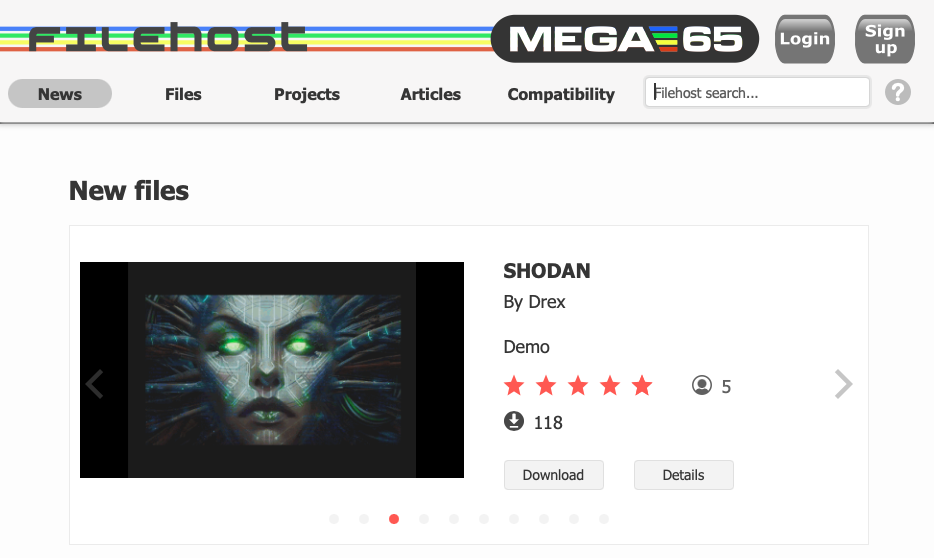
\includegraphics[width=0.7\linewidth]{images/filehost_notsignedin.png}}
\end{center}

Om een Filehost-account met uw eigenaarcode te registreren:

\begin{enumerate}
  \item Bezoek \href{https://files.mega65.org}{de Filehost-website}. Klik op ``Sign Up''. Volg de aanwijzingen om een account aan te maken.  \item Zoek uw eigenaarcode op.\index{Eigenaarscode} Dit is een code die op een papiertje staat afgedrukt; het papiertje was bij uw MEGA65 inbegrepen (mogelijk is het in deze handleiding gestoken). De code ziet er ongeveer als volgt uit: {\tt 123-ABC-456}  \item Klik in de rechterbovenhoek van het Filehost-scherm op het gebruikerspictogram. Selecteer in het pop-upmenu ``Redeem Code''. Voer uw eigenaarcode in zoals gevraagd.
\end{enumerate}

\begin{center}
  \fbox{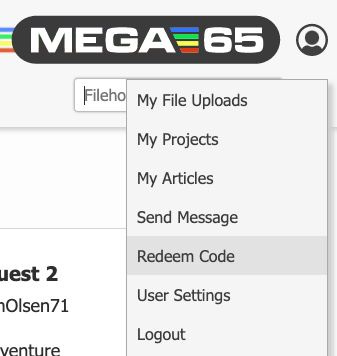
\includegraphics[width=0.4\linewidth]{images/filehost_redeemmenu.png}}
\end{center}

Om het nieuwste releasepakket te downloaden:

\begin{enumerate}
  \item Klik op het tabblad ``Files'' van de Filehost-website.  \item Typ in het zoekvak aan de linkerkant: ``core release''. De lijst wordt bijgewerkt en toont vervolgens alleen bestanden met deze woorden in de titel.  \item Zoek de vermelding genaamd ``MEGA65 Core Release Package (mega65r6) with ROM'', waarbij ``mega65r6'' overeenkomt met uw hardware-revisie. (Om uw hardware-revisie te bevestigen opent u het Freezer-menu en drukt u daarna op \specialkey{HELP}.)  \item Klik op de vermelding. Bevestig dat dit releasepakket voor uw hardware-revisie is en klik daarna op ``Download'' om het bestand te downloaden.
\end{enumerate}

\underline{OPMERKING}: Er bestaat een vermelding van het releasepakket zonder de ROM. Deze vermelding is voor iedereen zichtbaar. Om er zeker van te zijn dat u een compatibele set bestanden gebruikt, kiest u het pakket waarop ``with ROM'' staat. Indien u geen vermelding ziet waarop ``with ROM'' staat, controleer dan of u bent aangemeld en of u een geldige eigenaarcode heeft ingewisseld.

\begin{center}
  \fbox{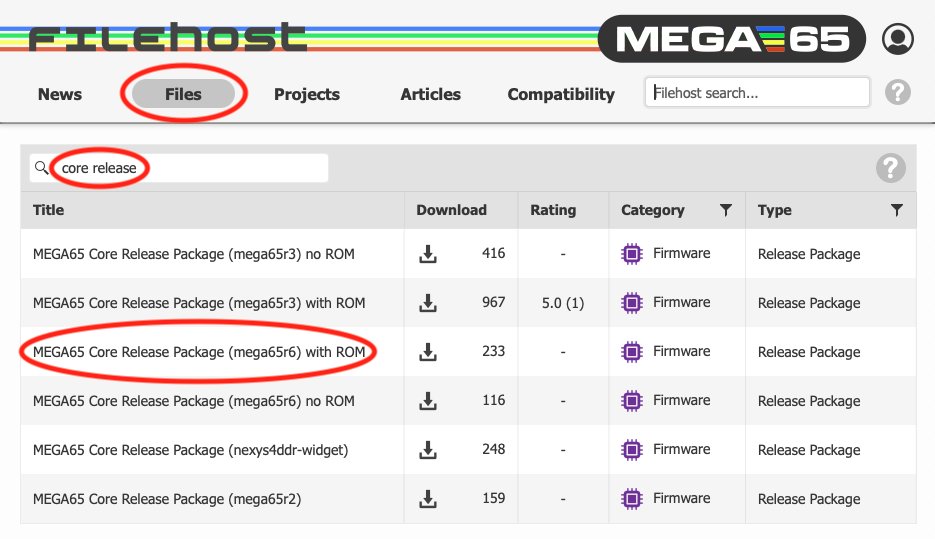
\includegraphics[width=0.7\linewidth]{images/filehost_release.png}}
\end{center}

Pak het gedownloade {\tt .7z}-archief uit. U zou een bestand moeten zien waarvan de naam eindigt op {\tt .cor} en een map {\tt sdcard-files} die een bestand bevat met de naam {\tt MEGA65.ROM}.

\section{Het corekeuzemenu}
\index{Core!Corekeuzemenu}

De MEGA65 bepaalt welke core bij het opstarten in de FPGA wordt geladen. U kunt dit proces onderbreken om te kiezen welke core wordt geladen.\footnote{Strikt genomen start de MEGA65 de core in slot 0 op om het corekeuzemenu te laten draaien. Nadat u een keuze hebt gemaakt of de computer een standaardcore kiest, laadt de computer de gekozen core in de FPGA en vervolgt hij het opstartproces.}

Om het corekeuzemenu te openen schakelt u de computer uit, houdt u de toets \specialkey{NO\\SCROLL} ingedrukt en schakelt u de computer weer in. Het corekeuzemenu verschijnt, met de acht coreslots, genummerd van 0 tot en met 7.

\begin{center}
  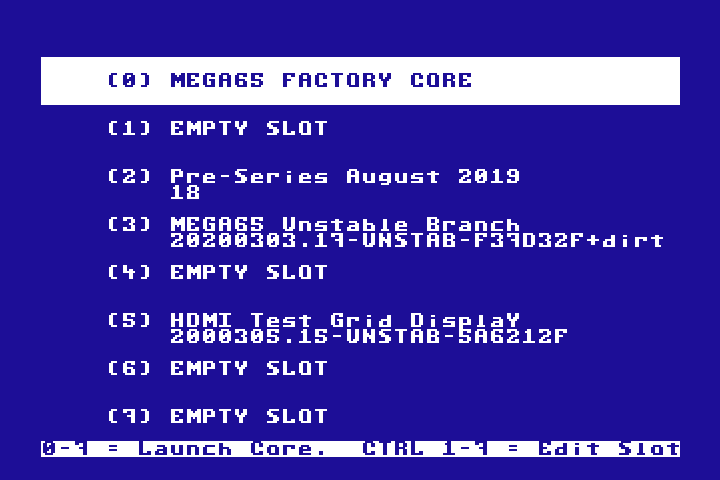
\includegraphics[width=0.7\linewidth]{images/ss-flashmenu.png}
\end{center}

U kunt met de cursortoetsen en \specialkey{RETURN} een core kiezen om op te starten, of u kunt eenvoudigweg de cijfertoets indrukken die overeenkomt met het slot. Het opstartproces wordt voortgezet met de nieuwe core. De MEGA65 blijft de nieuwe core gebruiken totdat u de computer uitschakelt. (Het indrukken van de resetknop wijzigt niet welke core wordt gebruikt.)

Wanneer u de computer inschakelt zonder het corekeuzemenu te openen, zoekt de MEGA65 naar een standaardcore. De computer controleert eerst of een core als standaardcore is gemarkeerd (een instelling die u kunt wijzigen). Indien geen enkele core zo is gemarkeerd, controleert de computer daarna of er een core in slot 1 staat.\footnote{Indien DIP-schakelaar \#4 in de stand ``on'' staat, controleert de MEGA65 slot 2 in plaats van slot 1. De DIP-schakelaars bevinden zich in de behuizing, op het moederbord.} Indien het slot leeg is, gebruikt de computer slot 0.

Uw computer is in de fabriek uitgerust met de MEGA65-core in slot 0. Wij raden u aan de in de fabriek geïnstalleerde core niet te upgraden, tenzij het MEGA65-team u dat adviseert. Installeer nieuwe versies van de MEGA65-core in plaats daarvan in slot 1.

\section{De core, ROM en systeembestanden upgraden}
\index{Core!Upgraden}\index{ROM!Upgraden}

Vanuit het corekeuzemenu kunt u een core upgraden of een nieuwe core installeren. Tijdens dit proces leest de computer het bestand {\tt .cor} van de SD-kaart.

Om de MEGA65-core, ROM en systeembestanden te upgraden:

\begin{enumerate}
  \item Verwijder de SD-kaart (of microSD-kaart) uit de MEGA65 en sluit deze met een SD-kaartlezer aan op uw PC.\footnote{In plaats van de SD-kaart naar uw PC over te brengen kunt u de bestanden ook via een Ethernet-verbinding overzetten. Zie hoofdstuk \vref{cha:transferring-files}.}  \item Kopieer het {\tt .cor}-bestand dat u uit het {\tt .7z}-archief hebt gehaald naar de SD-kaart.  \item Open op uw PC de map {\tt sdcard-files} uit het {\tt .7z}-archief en kopieer deze bestanden daarna naar de SD-kaart, waarbij u de bestaande bestanden vervangt. Plaats ze in de hoofdmap van het bestandssysteem van de SD-kaart, niet in een submap.  \item Werp de SD-kaart uit via het besturingssysteem van uw PC en plaats deze daarna terug in de MEGA65.  \item Open het corekeuzemenu: schakel de MEGA65 uit en houd daarna \specialkey{NO\\SCROLL} ingedrukt terwijl u de computer weer inschakelt.  \item Houd \specialkey{CTRL} ingedrukt en druk daarna op het cijfer van het slot dat u wilt upgraden. De sloteditor opent.  \item Druk op \megakey{F3} om een core-bestand te laden. De bestandsselectie opent. Gebruik de cursortoetsen om het {\tt .cor}-bestand te selecteren en druk daarna op \specialkey{RETURN}.  \item Druk op \megakey{F8} om het coreslot te flashen. Laat het flashen volledig verlopen. Dit duurt enkele minuten.  \item Wanneer het flashen is voltooid, drukt u op een willekeurige toets om terug te keren naar het corekeuzemenu.
\end{enumerate}

De sloteditor ziet er als volgt uit:

\begin{center}
  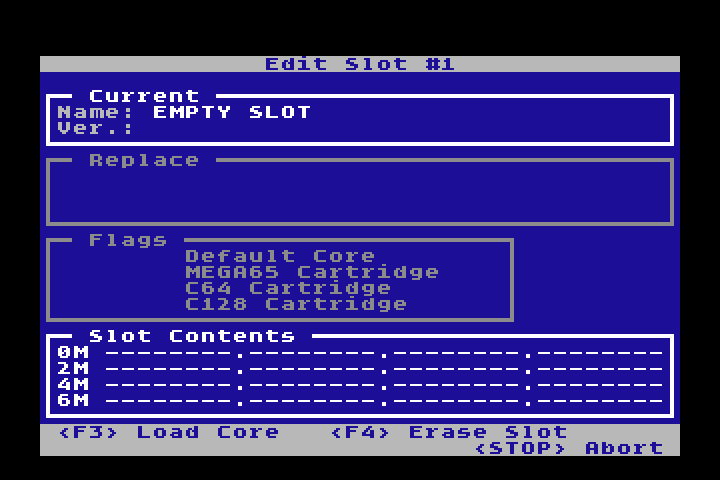
\includegraphics[width=0.7\linewidth]{images/ss-flashmenu-sloteditor.png}
\end{center}

Wanneer u een core-bestand laadt, vraagt de computer u het {\tt .cor}-bestand te selecteren op een scherm dat op dit voorbeeld lijkt:

\begin{center}
  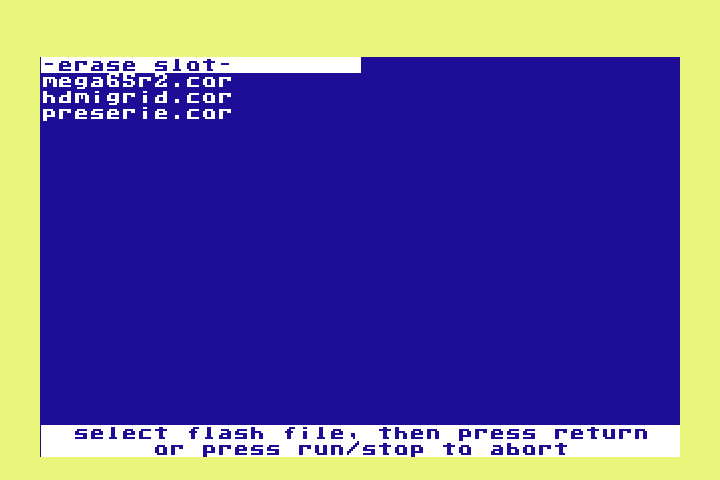
\includegraphics[width=0.7\linewidth]{images/ss-flashmenu-selectcore.png}
\end{center}

Nadat u de core hebt geselecteerd, toont de sloteditor welke wijziging deze in het slot wil aanbrengen. Wanneer u het flashen start, toont het beeldscherm de voortgang.

\underline{OPMERKING}: Schakel uw computer {\em niet} uit en onderbreek de stroomtoevoer niet voordat deze stap is voltooid.

\begin{center}
  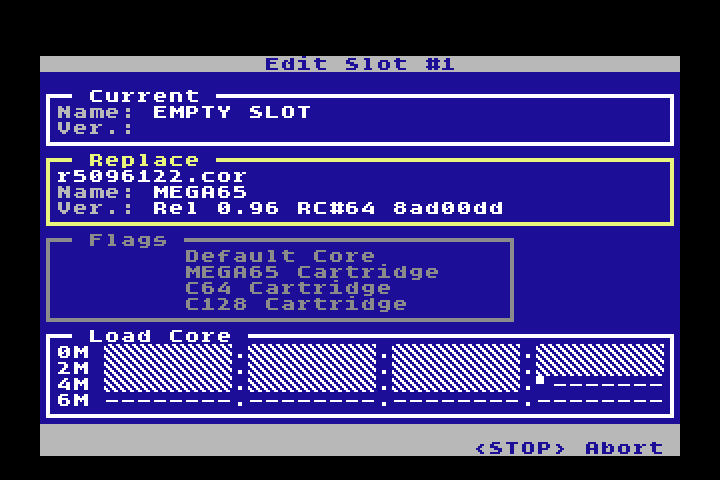
\includegraphics[width=0.7\linewidth]{images/ss-flashmenu-loading.png}
\end{center}

Wanneer de melding "Core was successfully flashed" wordt weergegeven, is het proces voltooid.

\begin{center}
  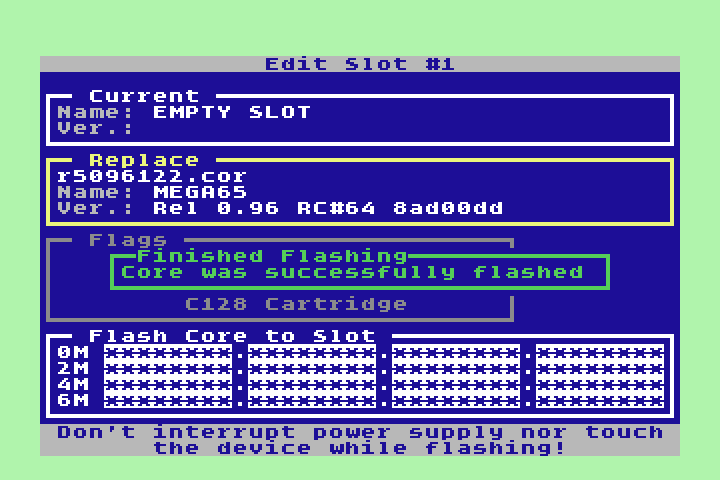
\includegraphics[width=0.7\linewidth]{images/ss-flashmenu-complete.png}
\end{center}

Het is nu veilig om uw computer uit te schakelen. Druk op een willekeurige toets om terug te keren naar het corekeuzemenu, of schakel de computer uit en daarna weer in om de standaardcore te starten.


\section{Alternatieve cores en ROM's installeren}

Het installeren van een alternatieve core, zoals de C64-core,\index{Core!C64-core} verloopt volgens dezelfde stappen voor het flashen van de core naar een slot.

Het is raadzaam de slots 2 tot en met 7 voor alternatieve cores te gebruiken en slot 1 voor de nieuwste MEGA65-core te reserveren. Er staat u uiteraard niets in de weg om een alternatieve core in slot 1 te installeren, zodat de MEGA65 zich bij het inschakelen als een ander type computer gedraagt. De MEGA65-core kunt u altijd kiezen via het corekeuzemenu.

U kunt meer dan één versie van de MEGA65-ROM op de SD-kaart bewaren. Wanneer u de MEGA65-core opstart, kunt u één van deze ROM's selecteren door tijdens het opstarten een cijfertoets ingedrukt te houden.

Om alternatieve ROM's te installeren kopieert u ze naar de hoofdmap van de SD-kaart, met een bestandsnaam zoals {\tt MEGA65x.ROM}, waarbij {\tt x} een getal tussen 0 en 8 is. Om de alternatieve ROM op te starten houdt u de bijbehorende cijfertoets ingedrukt terwijl de MEGA65-core start. Indien u geen cijfer ingedrukt houdt, start de computer standaard {\tt MEGA65.ROM} op.

Er zijn verschillende redenen waarom u alternatieve ROM's op uw SD-kaart zou willen bewaren:

\begin{itemize}
  \item U helpt een nieuwe bètaversie van de ROM te testen en u wilt de bètaversie niet tot uw standaard-ROM maken.
  \item U wilt de originele prototype-ROM van de Commodore 65 proberen. De MEGA65-core behoudt de achterwaartse compatibiliteit met de C65-ROM waaraan Commodore werkte voordat het bedrijf het project annuleerde. Deze ROM is gebrekkig en onvolledig, maar vormt nog steeds een interessant historisch artefact.
  \item U wilt een alternatieve ROM proberen die door de MEGA65-gemeenschap is ontwikkeld. Eén van deze ROM's is de MEGA65 OpenROM, een project om een volledig nieuwe ROM te maken die onder een open-sourcelicentie wordt uitgebracht, zonder enig oorspronkelijk Commodore-materiaal.
\end{itemize}

Bij uw MEGA65-SD-kaart werden diverse alternatieve ROM's meegeleverd, die in de fabriek zijn geïnstalleerd. Probeer uw computer opnieuw op te starten terwijl u een cijfertoets ingedrukt houdt en kijk wat er gebeurt!

\section{Core-vlaggen instellen}

Er zijn verschillende opties (``vlaggen'') die u voor een core in de core-editor kunt kiezen.

Om vlaggen voor een core te wijzigen bewerkt u het coreslot. Druk op de cijfertoets die overeenkomt met de vlag om de waarde ervan om te schakelen. Sla de vlaggen in het slot op door het resultaat te flashen: druk op \megakey{F8}. U kunt de vlaggen vóór het flashen van nieuwe coregegevens instellen, of u kunt alleen de nieuwe vlaginstellingen flashen zonder de coregegevens te vervangen.

Om een core in te stellen als de standaardcore, welke wordt gebruikt wanneer de MEGA65 wordt ingeschakeld zonder \specialkey{NO\\SCROLL} ingedrukt te houden, stelt u de vlag "Default core" in. Indien geen enkele core als standaardcore is ingesteld, wordt slot 1 als standaard gebruikt (of slot 2 indien DIP-schakelaar \#4 in de stand ``on'' staat).

De vlaggen "cartridge" bepalen welke core wordt geselecteerd wanneer er een cartridge in de expansiepoort aanwezig is. Zo kunt u op basis van het type cartridge een andere standaardcore kiezen. U kunt bijvoorbeeld de MEGA65-core instellen om MEGA65-cartridges af te handelen en een andere core om C64-cartridges af te handelen. Standaard handelt de MEGA65-core C64-cartridges af met behulp van de "GO64"-modus. Wellicht geeft u er de voorkeur aan dit te wijzigen en de C64-core te gebruiken die u afzonderlijk installeert.

\begin{center}
  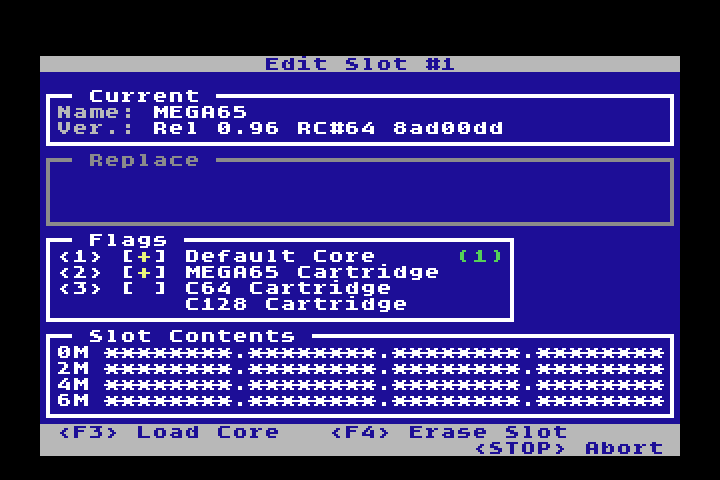
\includegraphics[width=0.7\linewidth]{images/ss-flashmenu-flags.png}
\end{center}

\section{Een coreslot wissen}

Het flashen vervangt wat er in een coreslot staat door de nieuwe core. Indien er al een core in het slot is geïnstalleerd, overschrijft het flashen de bestaande core.

Indien u een core wilt verwijderen en het slot leeg wilt laten, bewerkt u het slot en drukt u op \megakey{F4} om de vervanging in te stellen op "Erase slot". Druk daarna op \megakey{F8} om het slot met lege gegevens te flashen.

\section{De fabriekscore in slot 0 upgraden}
\index{Core!Fabriekscore in slot 0 upgraden}

Het is mogelijk de in de fabriek geïnstalleerde MEGA65-core in slot 0 te upgraden. Dit hoeft u alleen in zeldzame gevallen te doen, bijvoorbeeld indien een nieuwere versie van de MEGA65-core wijzigingen of foutcorrecties voor het opstartproces bevat. Het is raadzaam slot 0 niet te upgraden, tenzij de aankondiging van de uitgave daartoe aanleiding geeft. De meeste upgrades van de MEGA65-core zijn in slot 1 volledig functioneel, zonder dat u slot 0 hoeft te upgraden.

Het is belangrijk dat ten minste één coreslot een werkende MEGA65-core bevat. Indien er tijdens het flashen iets misgaat, kan dit leiden tot een niet-werkende core in dat slot. Om ongelukken te helpen voorkomen verschilt de procedure voor het flashen van slot 0 enigszins van die van de andere slots en kan alleen een officiële MEGA65-core naar slot 0 worden geflasht.

{\em Lees deze aanwijzingen zorgvuldig door voordat u met de procedure begint.} Om de core in slot 0 te upgraden:

\begin{enumerate}
  \item Installeer de nieuwste MEGA65-core in slot 1 met behulp van de hierboven beschreven procedure. De core moet zich in het standaardslot ongelijk aan nul bevinden om van eventuele problemen bij het upgraden van slot 0 te kunnen herstellen.  \item Start coreslot 1 op om te bevestigen dat het werkt.  \item Keer terug naar het corekeuzemenu: schakel de MEGA65 uit en houd daarna \specialkey{NO\\SCROLL} ingedrukt terwijl u de computer weer inschakelt.  \item Houd \megasymbolkey ingedrukt en druk op de komma-toets om de editor voor slot 0 te openen.  \item Lees het informatiescherm en typ daarna het woord {\tt CONFIRM} in hoofdletters en druk op \specialkey{RETURN}.  \item Herhaal de rest van de flashprocedure om het core-bestand te selecteren en het slot te flashen.
\end{enumerate}

\underline{OPMERKING}: Indien u een MEGA65 van revisie R3A heeft en slot 0 nog niet eerder heeft geüpgraded, starten \megasymbolkey en de komma-toets de procedure niet: u heeft een oudere core in slot 0 die deze voorziening niet heeft. U kunt dit omzeilen door het corekeuzemenu opnieuw te starten met slot 1. Bereid u vanuit het corekeuzemenu voor om \specialkey{NO\\SCROLL} ingedrukt te houden, druk op \megakey{1} om de core op te starten en druk daarna onmiddellijk op \specialkey{NO\\SCROLL} en houd deze ingedrukt. Het corekeuzemenu wordt daarna opnieuw geopend met behulp van slot 1. Druk op \megasymbolkey en de komma-toets om de upgrade van slot 0 te voltooien.

Indien er tijdens het flashen van slot 0 iets misgaat, start uw MEGA65 mogelijk niet correct op. Schakel uw MEGA65 vóór al het andere in en wacht ongeveer een minuut. Na enige tijd zou de computer moeten merken dat er geen geldige core in slot 0 staat en vervolgens de core in slot 1 starten. U kunt tijdens dit proces \specialkey{NO\\SCROLL} ingedrukt houden om het corekeuzemenu van slot 1 te openen en het flashen opnieuw te starten.

Indien de MEGA65 na enkele minuten nog geen enkele core kan opstarten, is de computer mogelijk vastgelopen. U kunt de computer wellicht herstellen met behulp van een apparaat dat een ``JTAG-interface'' heet en uw PC met het moederbord van de MEGA65 verbindt. Hiermee kunt u een bitstream rechtstreeks in de FPGA injecteren. Het onderdeel is goedkoop, doch niet altijd verkrijgbaar. Neem voor hulp contact op met het MEGA65-team via de Discord (\url{https://mega65.org/chat}).

Aan coreslot 0 kunnen geen vlaggen worden toegewezen, zoals een vlag om als standaardcore te dienen of om aan cartridgetypen te worden gekoppeld. Slot 0 wordt voor deze doeleinden gebruikt indien er geen andere core is geïnstalleerd. Het is raadzaam de nieuwste MEGA65-core in slot 1 te bewaren, naast het flashen van slot 0.


\section{Het opstartproces van de core begrijpen}
\nopagebreak
Deze sectie vat samen hoe de MEGA65 kiest met welke core hij bij het inschakelen opstart. Het proces wordt weergegeven in de volgende afbeelding:
\nopagebreak
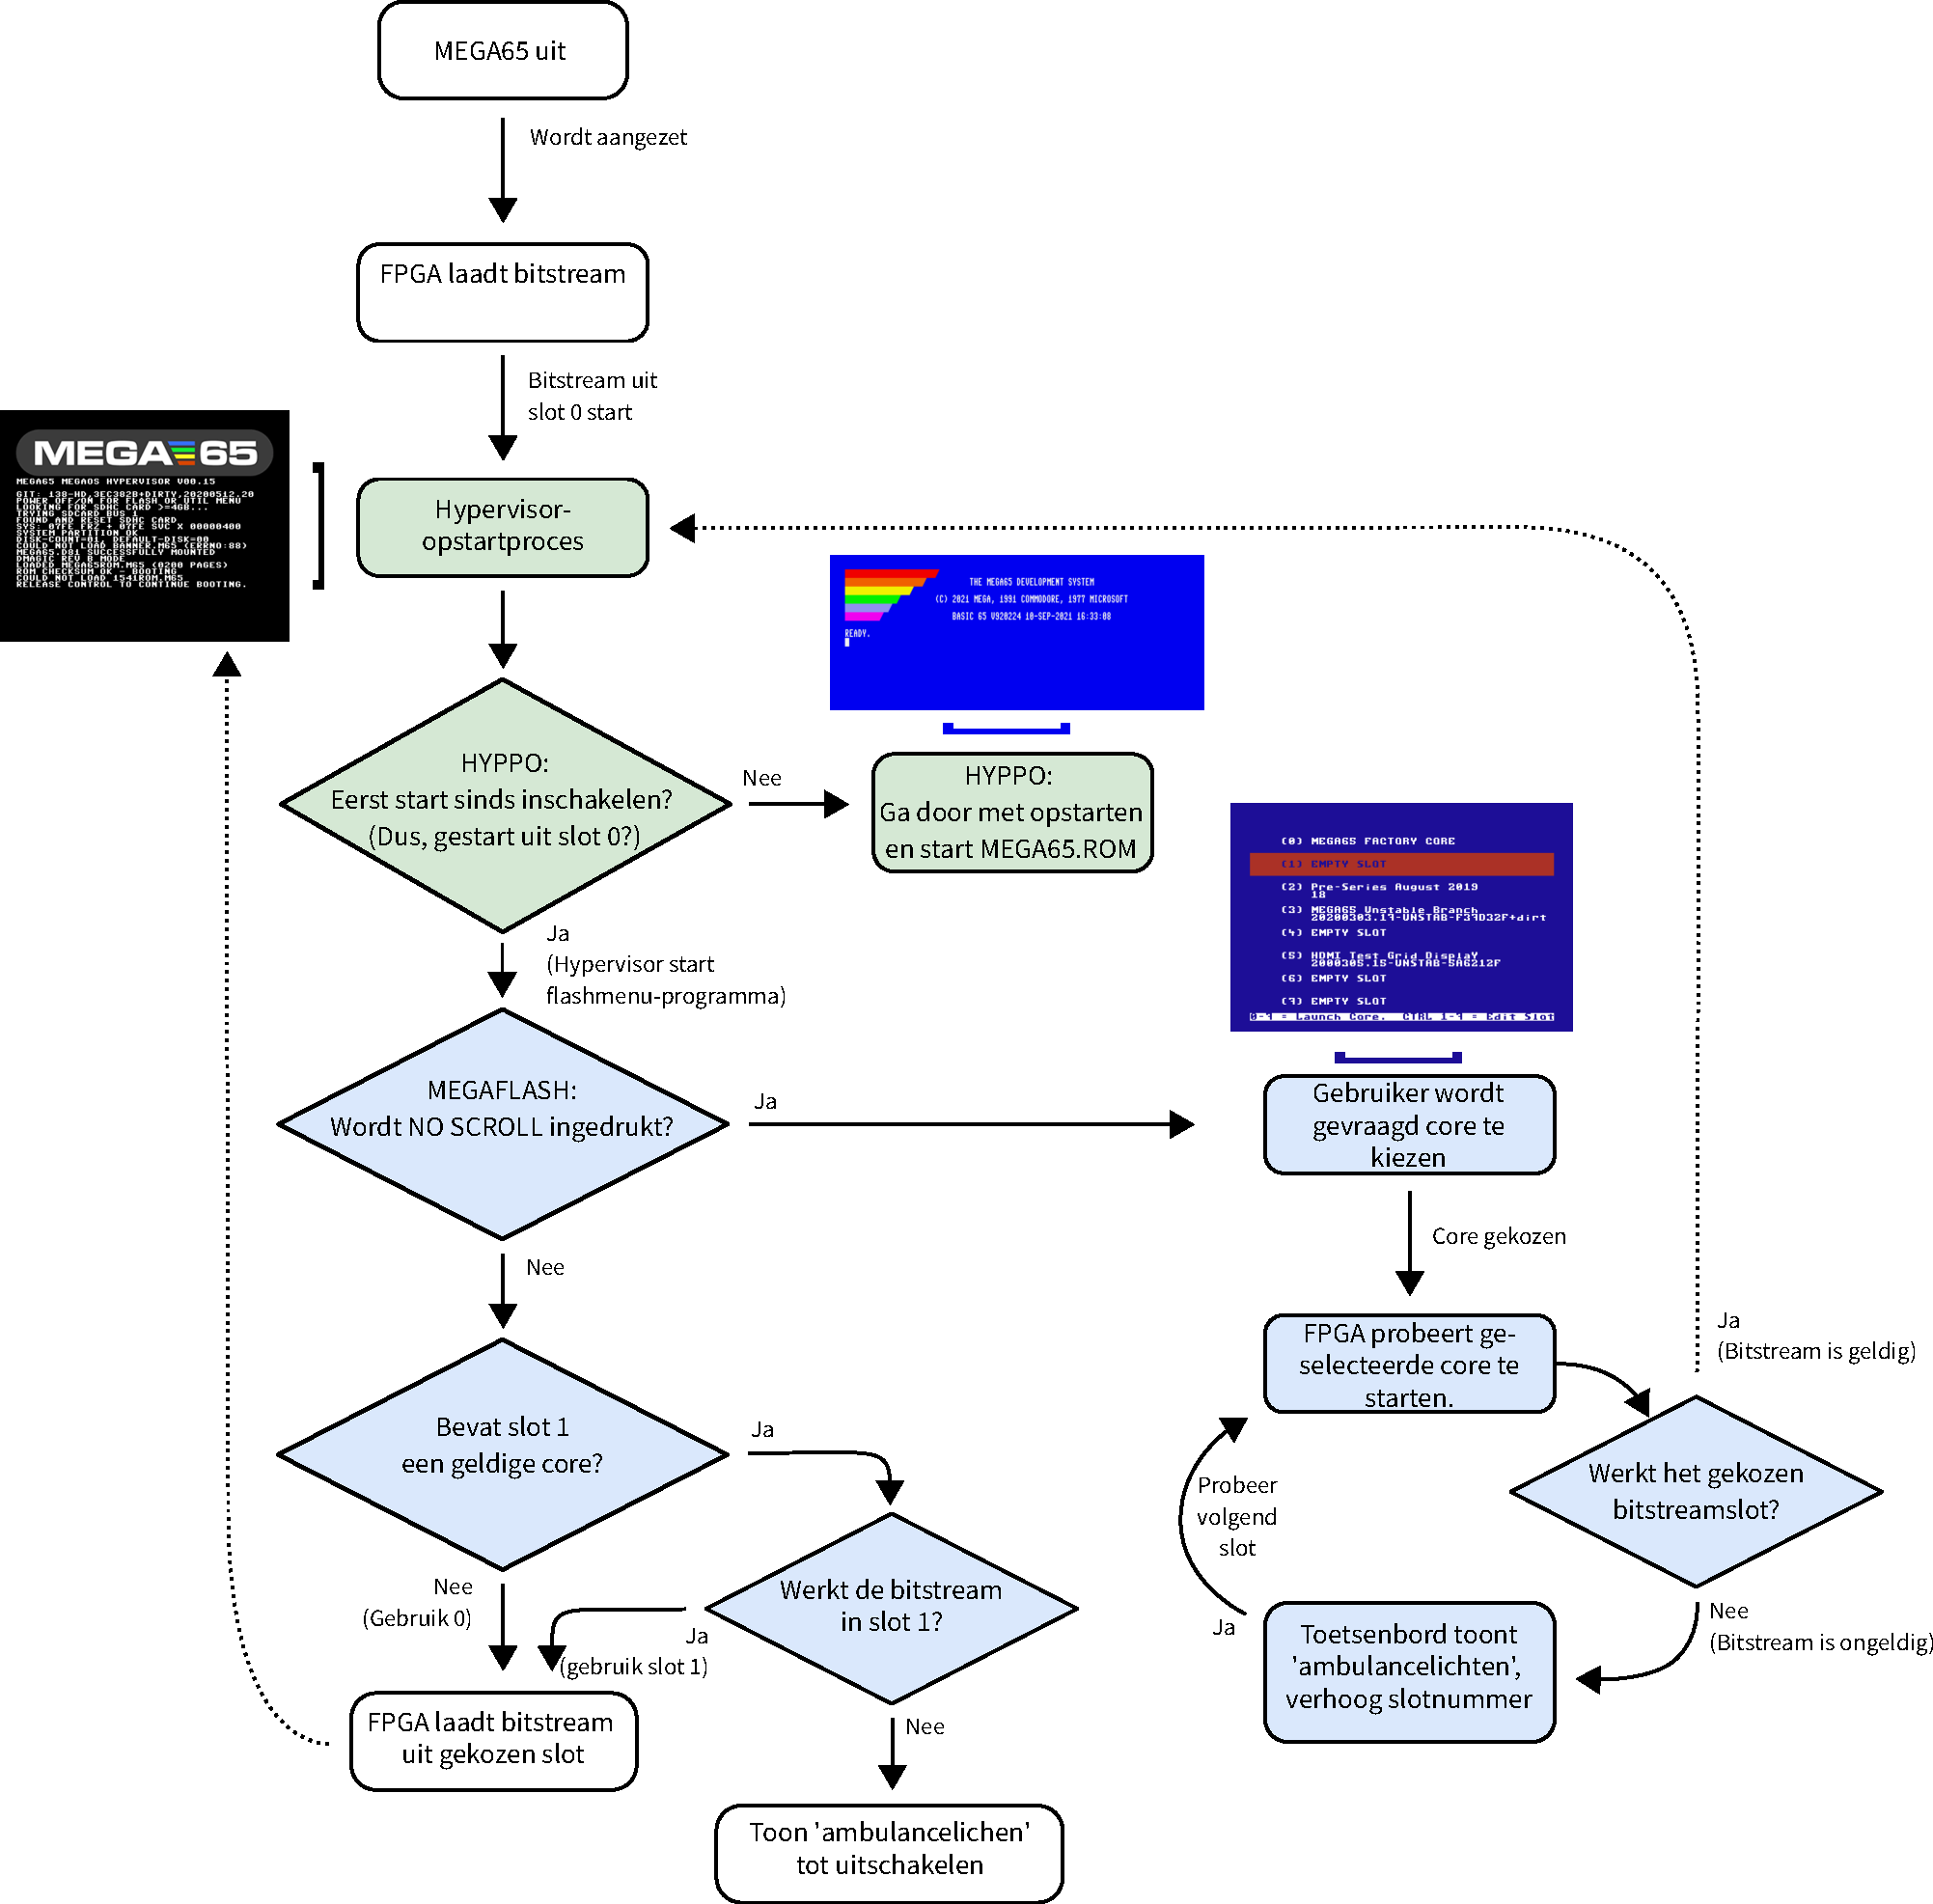
\includegraphics[width=\linewidth]{dutch/images/illustrations/flashmenu-flowchart.pdf}

Het opstartproces wordt beheerd door twee voorzieningen:
\begin{itemize}
  \item De Hypervisor (ook bekend als HYPPO), welke op een niveau boven de KERNAL werkt. Eén van zijn taken is het beheren van delen van het opstartproces. Raadpleeg voor meer details over de Hypervisor
\ifdefined\printmanual
{\bf Het grote Mega65-boek}.
\else
 \bookvref{sec:hypervisor-mode}.
\fi
    In het diagram zijn de activiteiten die de Hypervisor uitvoert groen gemarkeerd.  \item Het corekeuzemenuprogramma (ook bekend als ``MegaFlash''), welke een lijst met beschikbare coreslots biedt om uit te kiezen. In het diagram zijn de activiteiten die MegaFlash uitvoert blauw gemarkeerd.
\end{itemize}

Wanneer de MEGA65 wordt ingeschakeld, doet de computer het volgende:
\begin{itemize}
\item De MEGA65 laadt de bitstream in slot 0 van het flashgeheugen. Indien dat de MEGA65-fabriekscore is, start de HYPPO-hypervisor van de MEGA65.\item Indien het de eerste opstart na het inschakelen is (wat betekent dat u vanuit slot 0 werkt), start HYPPO het Flash-menu-programma (ook wel MegaFlash genoemd) -- maar houd er rekening mee dat het Flash-menu in deze modus mogelijk niets op het scherm toont om aan te geven dat het draait!\item Het Flash-menu controleert vervolgens of \specialkey{NO\\SCROLL} ingedrukt wordt gehouden.\item Indien dat het geval is, toont het Flash-menu zijn scherm, zodat u een core kunt selecteren of opnieuw flashen.\item Indien \specialkey{NO\\SCROLL} {\em niet} wordt ingedrukt gehouden, controleert het Flash-menu of Flash-slot 1 een geldige core bevat.\item Indien dat zo is, probeert het Flash-menu die core te laden.\item Indien dit lukt, herconfigureert het systeem zichzelf voor die core, waarna het gedrag van het systeem overeenkomt met die core.\item Indien dit mislukt, schakelt het toetsenbord over naar de ``ambulancemodus'', waarbij blauwe lampjes knipperen om aan te geven dat er eerste hulp nodig is. Merk op dat de resetknop in de ambulancemodus geen effect heeft: u moet de MEGA65 uitschakelen en weer inschakelen.
\end{itemize}

Indien u in het corekeuzemenu een andere core hebt geselecteerd, verloopt het proces op vergelijkbare wijze, met dit verschil dat de ambulancelampjes slechts gedurende een beperkte tijd branden: de FPGA zoekt namelijk automatisch door het flashgeheugen totdat hij een geldige core vindt. Indien hij het einde van het flashgeheugen bereikt, start hij de MEGA65-fabriekscore opnieuw vanuit slot 0.
